%\documentclass[compress]{beamer}

\documentclass[12pt]{beamer}
\usepackage{etex}
\usetheme{CambridgeUS}
\setbeamertemplate{headline}{}
\usecolortheme{seahorse}
\definecolor{UniBlue}{RGB}{83,121,170}
\setbeamercolor{frametitle}{fg=UniBlue}
\setbeamertemplate{navigation symbols}{}
%\setbeamercolor{itemize item}{fg=red}
%\beamertemplatenavigationsymbolsempty
%\setbeamertemplate{navigation symbols}{}
%\useoutertheme{default}

\usepackage{makeidx}  % allows for indexgeneration
\usepackage{mathtools} %
\usepackage{booktabs} %
\usepackage{verbatim} %
\usepackage{graphicx} %
\usepackage[labelformat=empty]{caption}
\usepackage{amsmath}
\usepackage{amssymb}
\usepackage{amsthm}
\usepackage{xspace}
\usepackage{multirow}
\usepackage{subfig}
\usepackage{pifont}
\usepackage{empheq}
\usepackage{relsize}
\usepackage{slashbox}
\usepackage{textcomp}
\usepackage{picture}
\usepackage{float}
\usepackage{url}
\usepackage{tikz}

%\usepackage[latin1]{inputenc}
%\usefonttheme{professionalfonts}
%\usepackage{times}
%\usetikzlibrary{arrows,shapes}

\usepackage[T1]{fontenc}
\usepackage{algorithmic} 
\usepackage{xparse}
%\usepackage[backend=bibtex,style=authortitle]{biblatex}
\usepackage[backend=bibtex,style=authortitle-ibid]{biblatex}
%\usepackage[backend=bibtex,style=mla]{biblatex} 
\addbibresource{present-bibli.bib}
\renewcommand{\footnotesize}{\tiny}
% \usepackage{algpseudocode} 
%\usepackage{algorithm}
%\usepackage[vlined]{algorithm2e} 

\usetikzlibrary{calc}

% tikzmark command, for shading over items
\newcommand{\tikzmark}[1]{\tikz[overlay,remember picture] \node (#1) {};}


\makeatletter
% \cvhrulefill{<color>}{<thickness>}
\newcommand*\cvhrulefill[2]{%
  \leavevmode\color{#1}\leaders\hrule\@height#2\hfill \kern\z@\normalcolor}
% \crule{<color>}{<width>}{<thickness>}
\newcommand*\crule[3]{%
  \color{#1}\rule{#2}{#3}\normalcolor}
\makeatother

\author{{\normalsize Emre Sefer \and Geet Duggal}
  \\ 
\vspace{0.65cm}
%{Carnegie Mellon University} \\
\vspace{1.75cm}

\includegraphics[width=2.0cm]{cmulogo.jpeg} \hspace{5cm} 
\includegraphics[width=1.5cm]{cpcblogo.jpeg}}

%\title{{\bf \large Deconvolution Of Ensemble Chromatin Interaction Data Reveals The Latent Mixing Structures In Cell Subpopulations}}
\title{{\bf \large Hi-C Topological Domains Tutorial}}

\normalsize

\newcommand{\FD}{\emph{3CDE}\xspace}
\newcommand{\FDfrac}{\emph{3CDEfrac}\xspace}
\newcommand{\FDint}{\emph{3CDEint}\xspace}%
\newcommand{\FDfracilp}{\emph{3CDEfrac}-opt\xspace}
\newcommand{\FDintilp}{\emph{3CDEint}-opt\xspace}
\newcommand{\Armatus}{\emph{Armatus}\xspace}
\newcommand{\Baseline}{$\emph{Armatus}_{\emph{Base}}$\xspace}
\newcommand{\MCMC}{\emph{MCMC5C}\xspace}
\newcommand{\BACHMIX}{\emph{BACHMIX}\xspace}
\newcommand{\HeLa}{\emph{HeLa}\xspace}
\newcommand{\Caulobacter}{\emph{Caulobacter}\xspace}
\newcommand{\CD}{\emph{CD$4^{+}$}\xspace}
\newcommand{\BQC}{\emph{BQC}\xspace}

\makeatletter
\def\overUnderArrow{\@ifnextchar[\overUnderArrow@i{\overUnderArrow@i[]}}
\def\overUnderArrow@i[#1]#2#3{% #1 under #2 over #3 main argument
  \ifx\relax#1\relax\array[b]{c}\overset{\text{#2}}{\uparrow}\\#3\endarray
  \else\ifx\relax#2\relax
    \array[t]{c}#3\\\underset{\text{#1}}{\downarrow}\endarray
  \else
    \array{c}\overset{\text{#2}}{\uparrow}\\#3\\\underset{\text{#1}}{\downarrow}\endarray
  \fi\fi}
\makeatother

\definecolor{Green}{rgb}{0,0.5,0}

\newcommand*{\boxedcolor}{red}
\makeatletter
\renewcommand{\boxed}[1]{\textcolor{\boxedcolor}{%
  \fbox{\normalcolor\m@th$\displaystyle#1$}}}
\makeatother

\begin{document}

%\captionsetup[figure]{labelformat=empty}
\setbeamertemplate{footline}{} 
\date{}

{\usebackgroundtemplate{%
%\tikz\node[opacity=0.2]{\includegraphics[height=\paperheight,width=\paperwidth]{tcot.png}};}
\tikz\node[opacity=0.2]{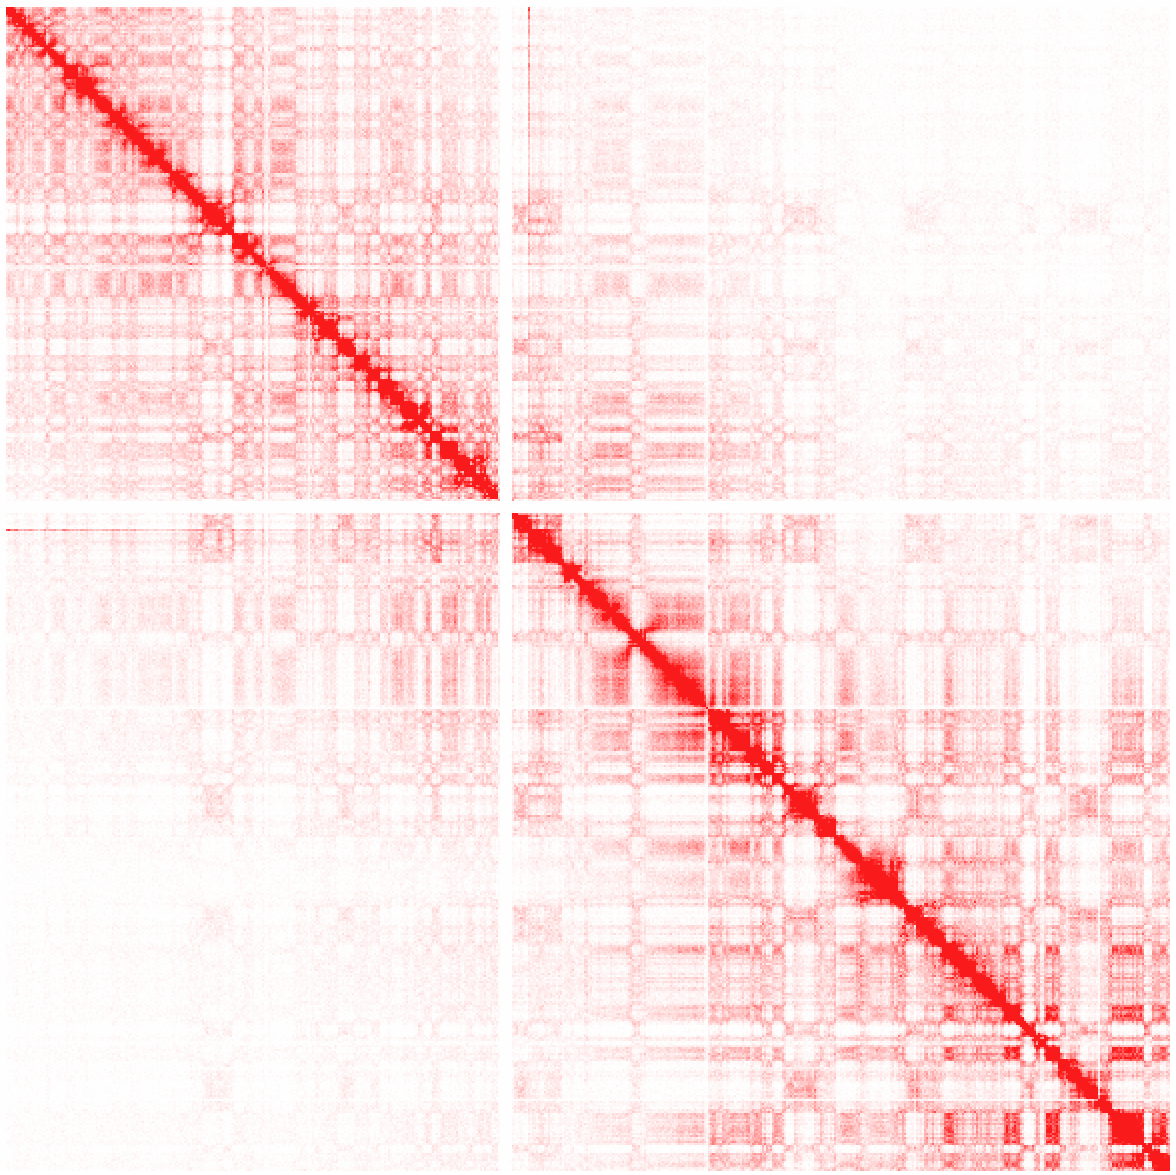
\includegraphics[height=0.9\paperheight,width=0.9\paperwidth]{hicpic2.png}};}
\frame{\titlepage}}


\begin{frame}
\frametitle{What are Topological Domains?}


\end{frame}


\begin{frame}
\frametitle{Chromatin Classification by PCA}

%\begin{figure}
%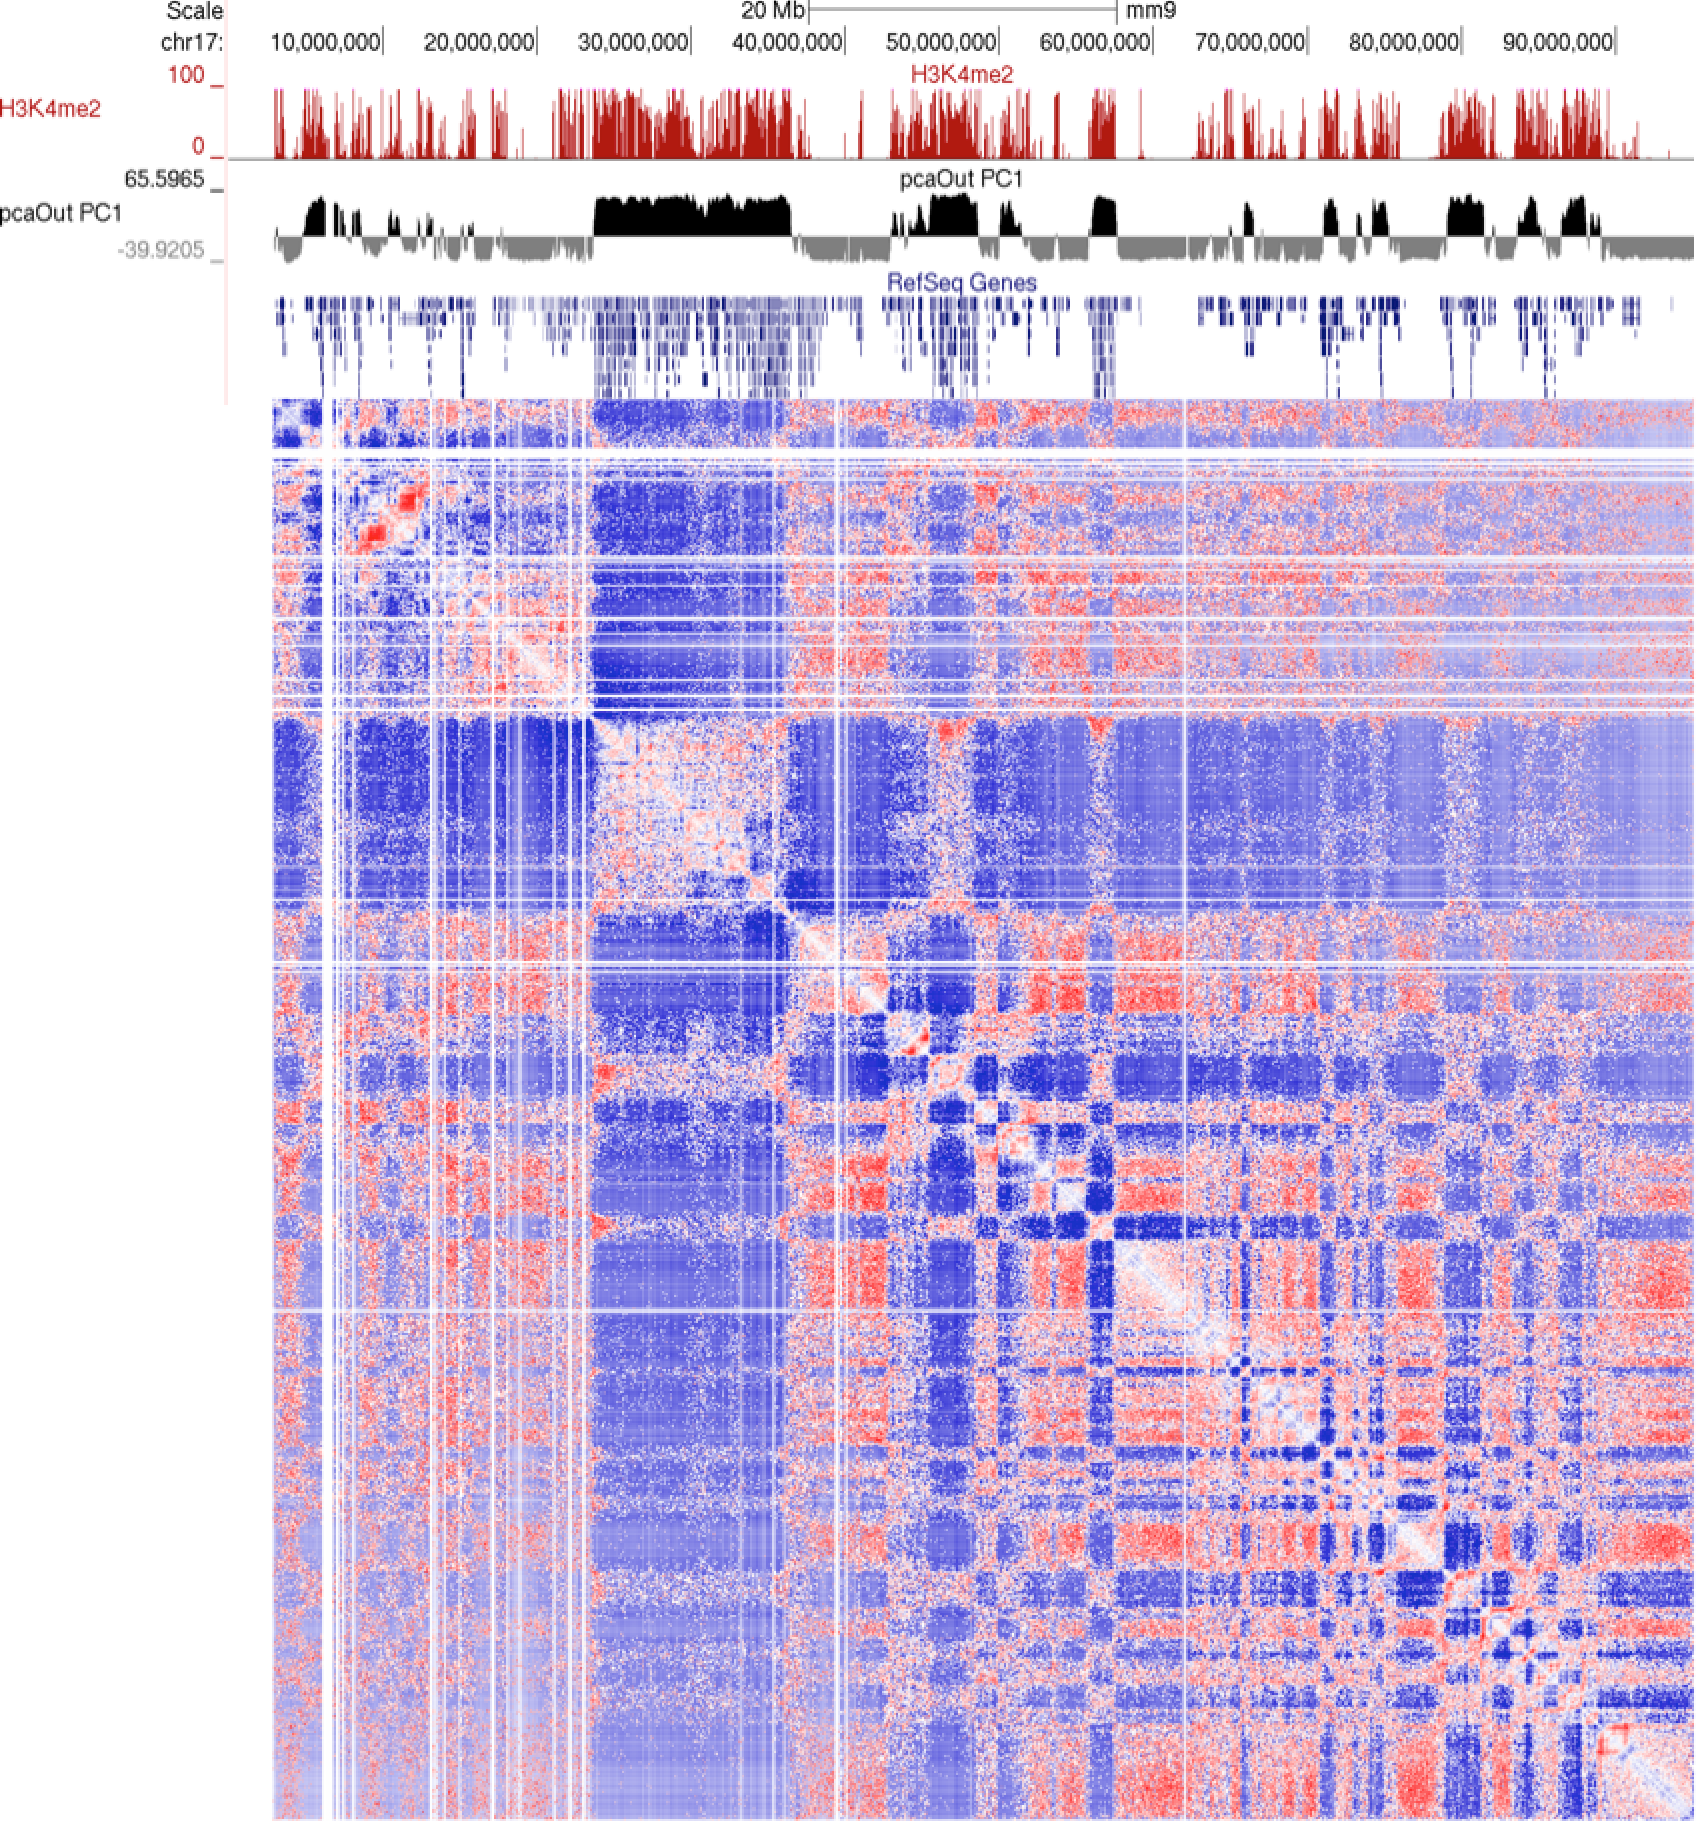
\includegraphics[scale=0.07]{pcamatrix.png}
%\end{figure}
\begin{figure}
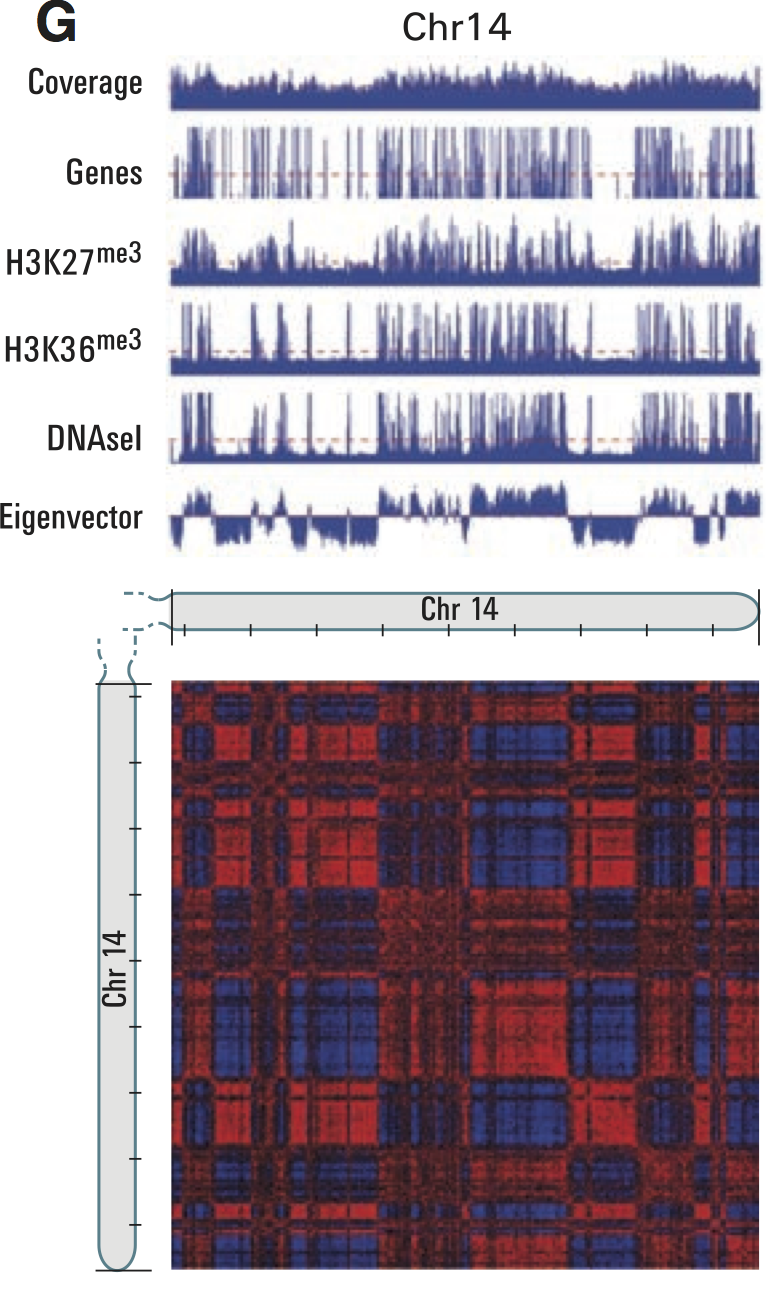
\includegraphics[scale=0.46]{eigen.png}
\end{figure}

%Classification of genomic domains with respect to gene activity, function, and nuclear
%compartments
\begin{itemize}
\item Human chromosomes are partitioned into two types of
  compartments:
\begin{itemize}
\item Compartment A -> open chromatin -> active gene-dense regions 
\vspace{0.07cm}
\item Compartment B -> closed chromatin -> repressive gene-poor regions
\end{itemize}
\end{itemize}

\footcitetext{aiden}

\end{frame}


\begin{frame}
\frametitle{TADs Are Enriched For Genomic Features}

\begin{figure}
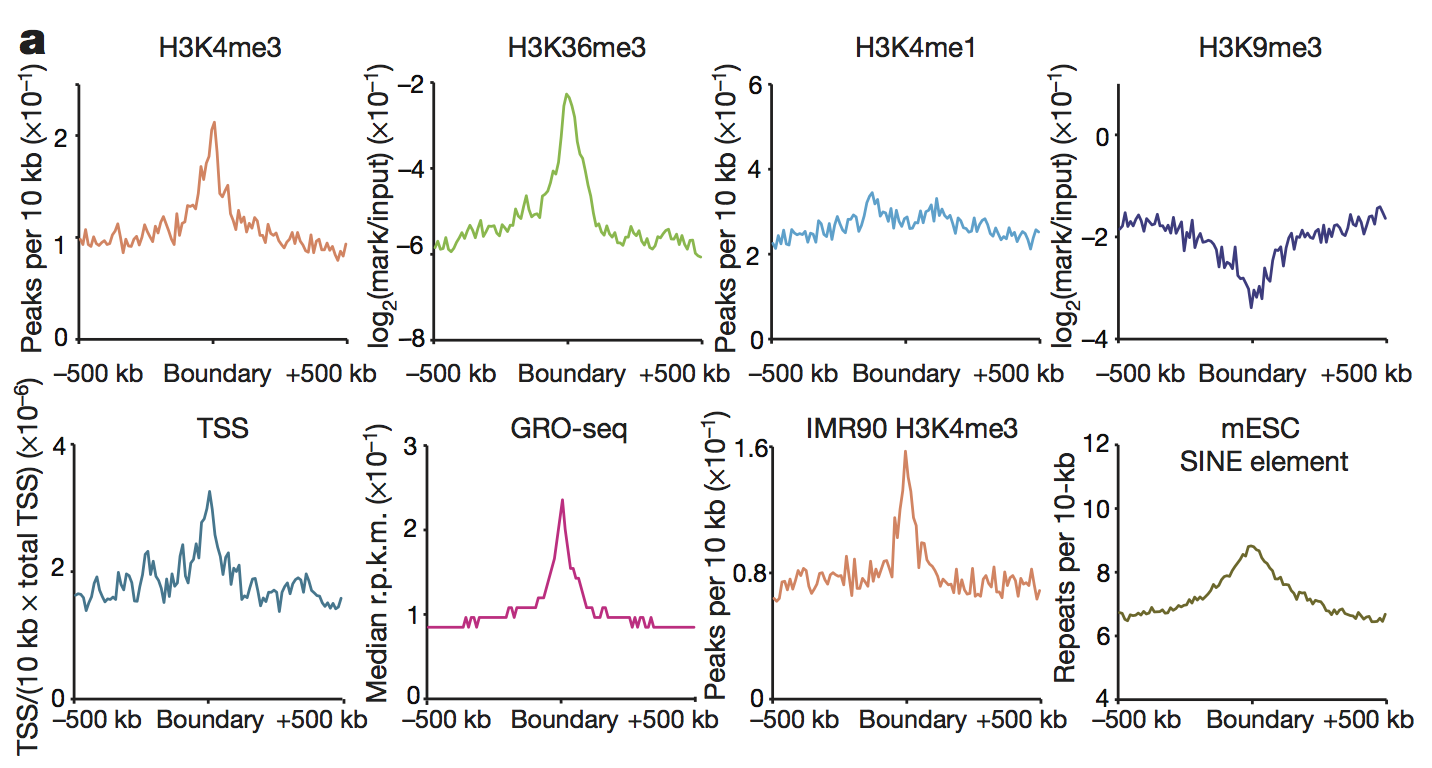
\includegraphics[scale=0.85]{feature.png}
\end{figure}

\begin{itemize}
\item H3k4me3 is enriched at TAD boundaries.
\vspace{0.1cm}
\item Repressive markers such as H3k9me3 are depleted at TAD boundaries.
\vspace{0.1cm}
\item CTCF binding sites are also enriched. 
\end{itemize}

\footcitetext{dixon2012}

\end{frame}


\begin{frame}
\frametitle{Domain Finder: Sexton et al.}

%Sexton et al. Need to determine main idea. Probability/likelihood (need to look into objective and algo) (E​mre)​
\begin{figure}
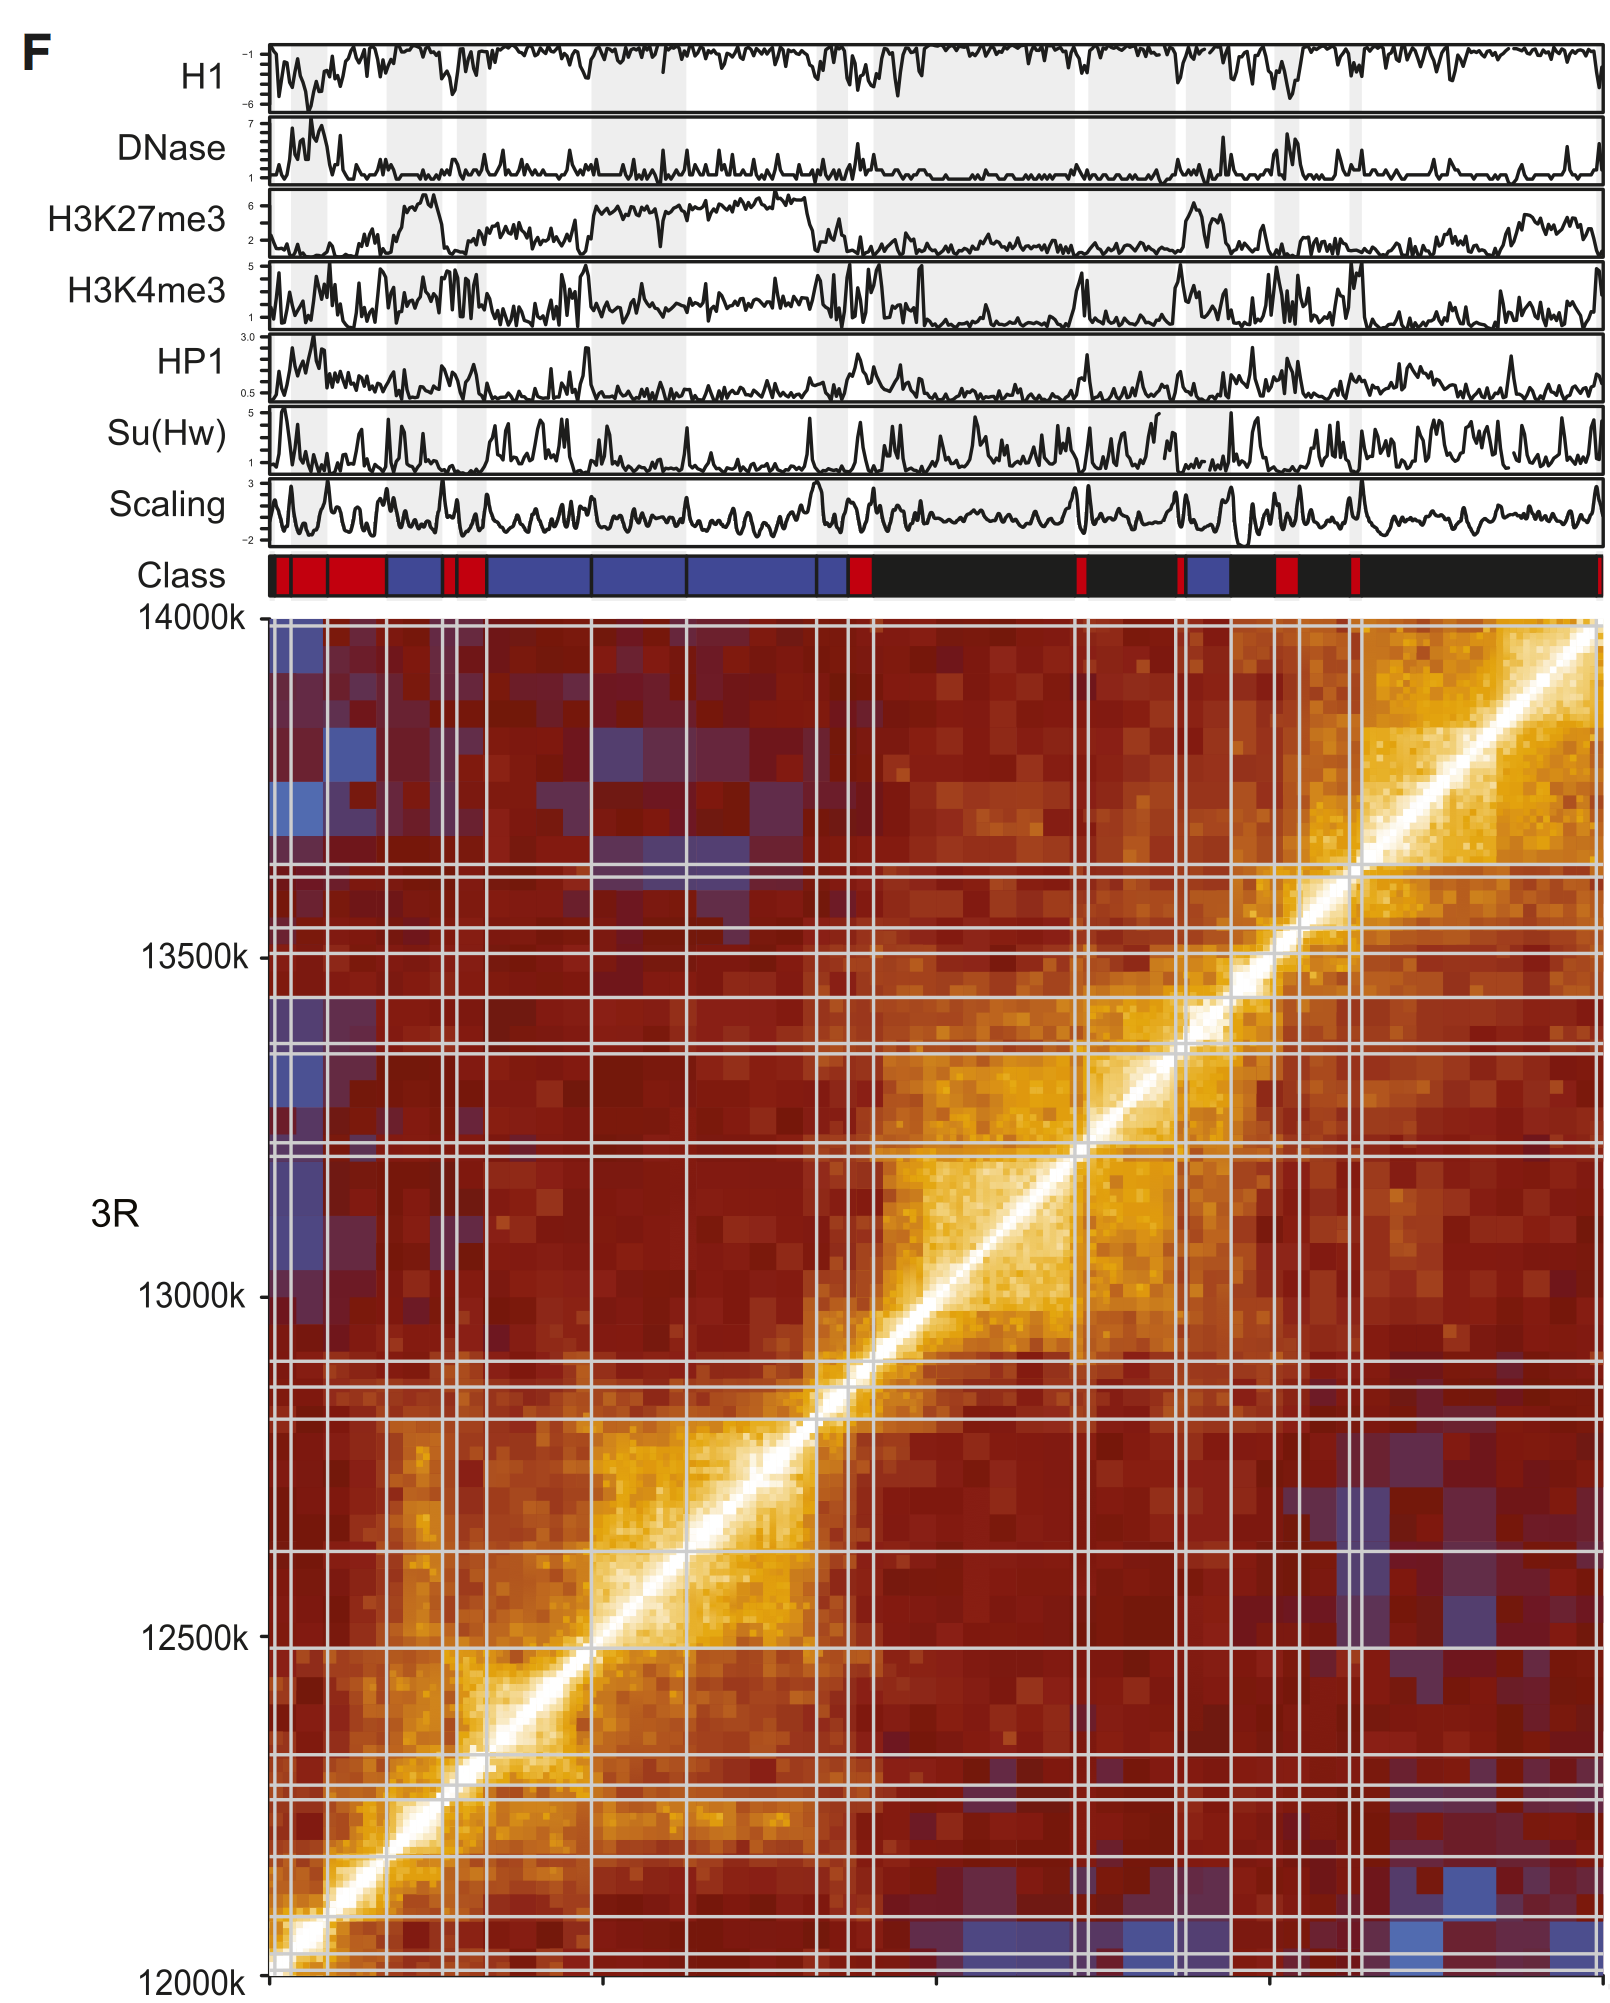
\includegraphics[scale=0.3]{dixon.png}
\end{figure}

\begin{itemize}
\item Domain partition based on likelihood optimization
\begin{figure}
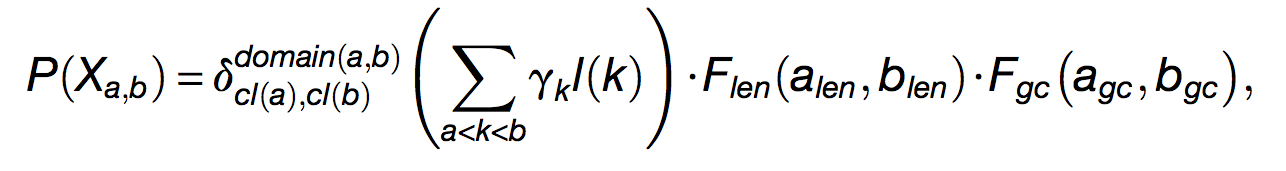
\includegraphics[scale=0.8]{dixoneq.png}
\end{figure}
\vspace{0.1cm}
\item Model parameters are estimated independently for each chromosome
\end{itemize}

\footcitetext{sexton2012}

\end{frame}


\begin{frame}
\frametitle{Domain Finder: Arrowhead}

\begin{figure}
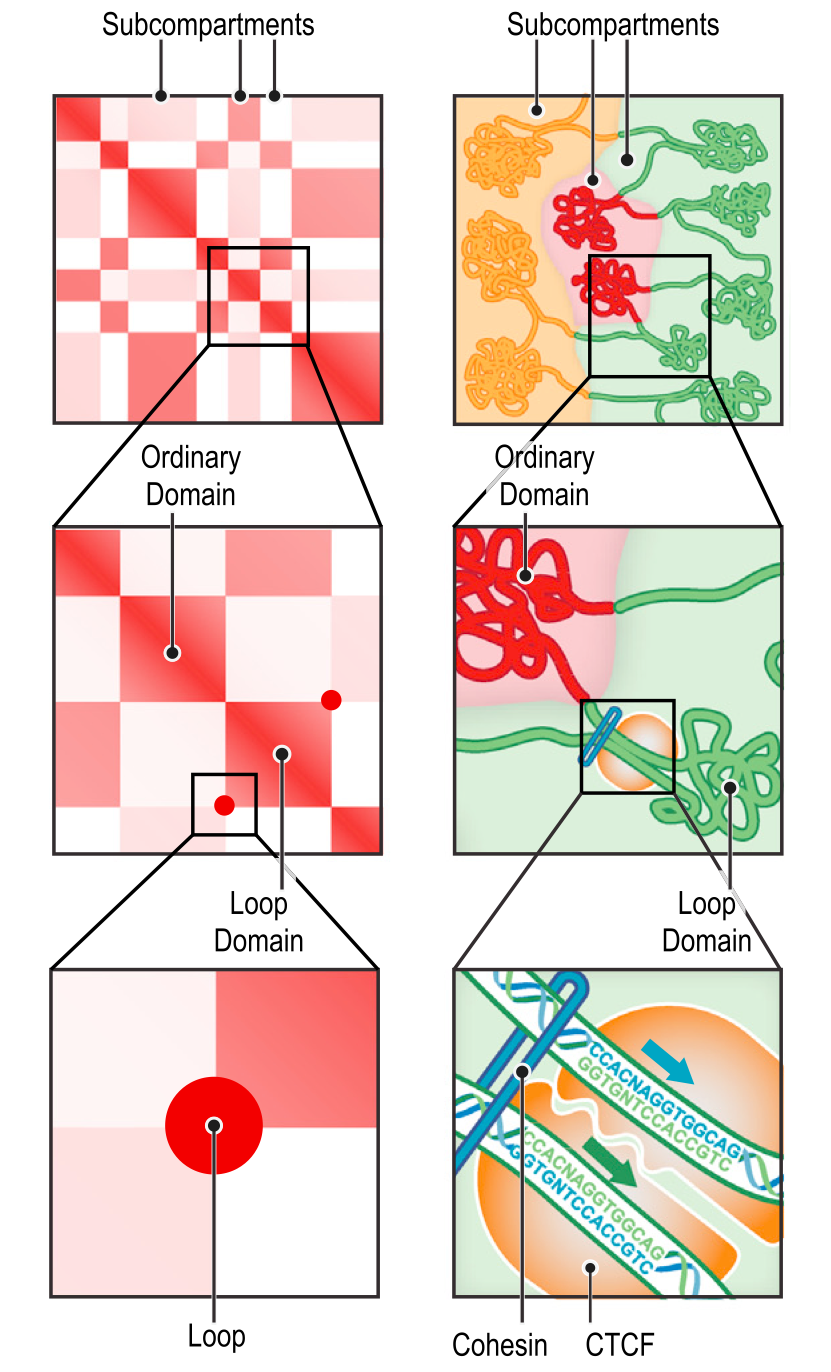
\includegraphics[scale=0.4]{arrowhead.png}
\end{figure}

\begin{itemize}
\item Arrowhead estimates a modified difference matrix $A$ varying between positive
  and negative values
\begin{itemize}
\item $A_{i, i+d}$ is strongly positive if locus $i-d$ is inside a domain
and locus $i+d$ is not.
\vspace{0.05cm}
\item $A_{i, i+d}$ is close to zero if both are inside a domain.
\end{itemize} 
\vspace{0.1cm}
\item Runs dynamic programming to find domains
\end{itemize}

\footcitetext{rao2014}

\end{frame}


\begin{frame}
\frametitle{Domain Finding via Deconvolution}

\begin{figure}
\includegraphics[scale=0.25]{decon_ex.png}
\end{figure}

\begin{itemize}
\item Given an ensemble Hi-C matrix, can we extract the mixing
  components?
\begin{itemize}
\item Identify TADs indirectly by deconvolution
\vspace{0.05cm}
\item Domains in the context of structural classes
\end{itemize}
\vspace{0.1cm}
\item Via combinatorial optimization
\end{itemize}

\footcitetext{decon2015}

\end{frame}


\begin{frame}
\frametitle{Domain Finder: TADBIT}

\begin{figure}
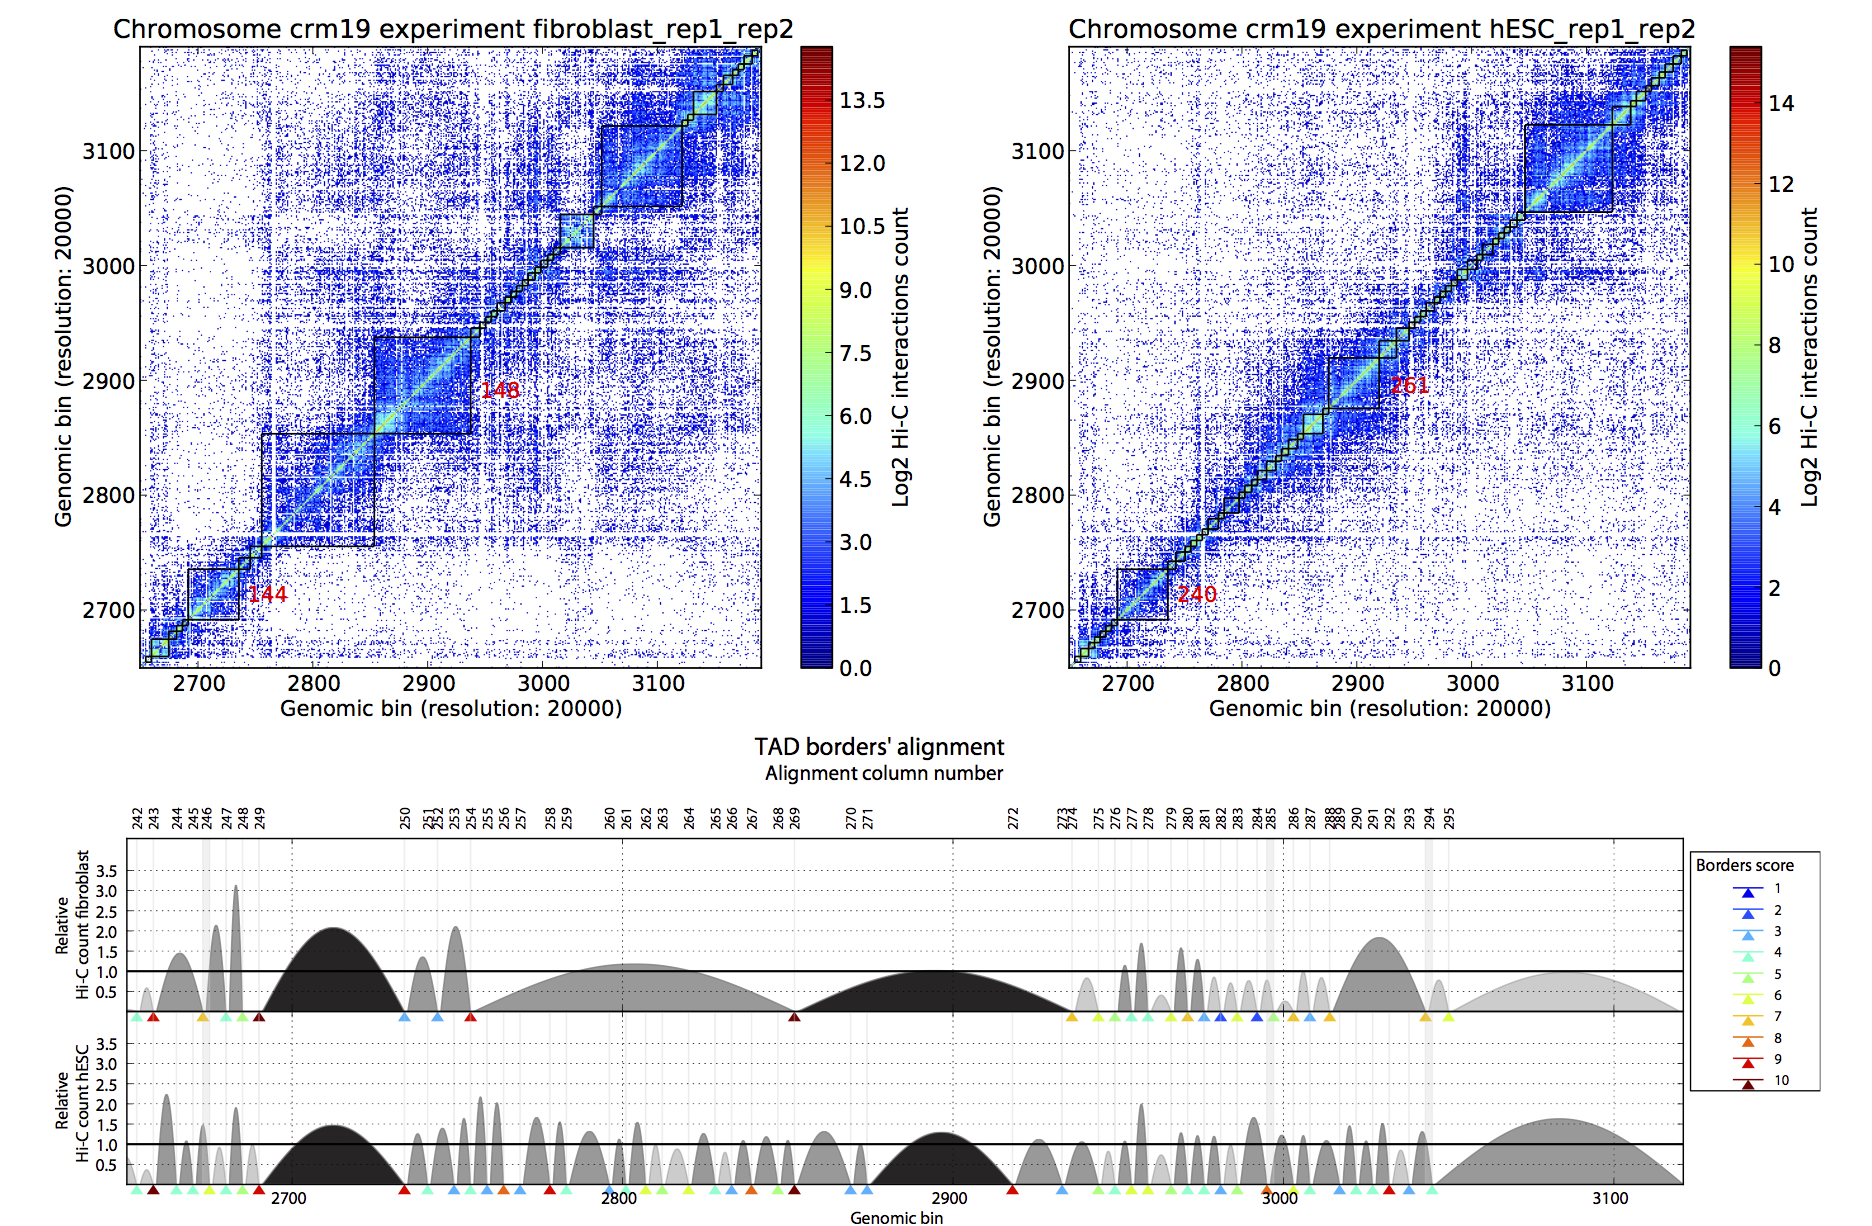
\includegraphics[scale=0.5]{tadbit.png}
\end{figure}

\begin{itemize}
\item TADBit uses breakpoint detection to detect TAD border positions
\begin{itemize}
\item It uses BIC penalized estimation of likelihood
\vspace{0.1cm}
\item Poisson assumption of Hi-C counts
\end{itemize}
\vspace{0.1cm}
\item Dynamic programming based algorithm
\end{itemize}

\footcitetext{tadbit}

\end{frame}


\begin{frame}
\frametitle{Disadvantages of the existing methods}


\end{frame}


% \begin{frame}
% \frametitle{Chromosome Conformation Capture~($3$C)}

% \begin{figure}
% \begin{minipage}{.47\textwidth}
% 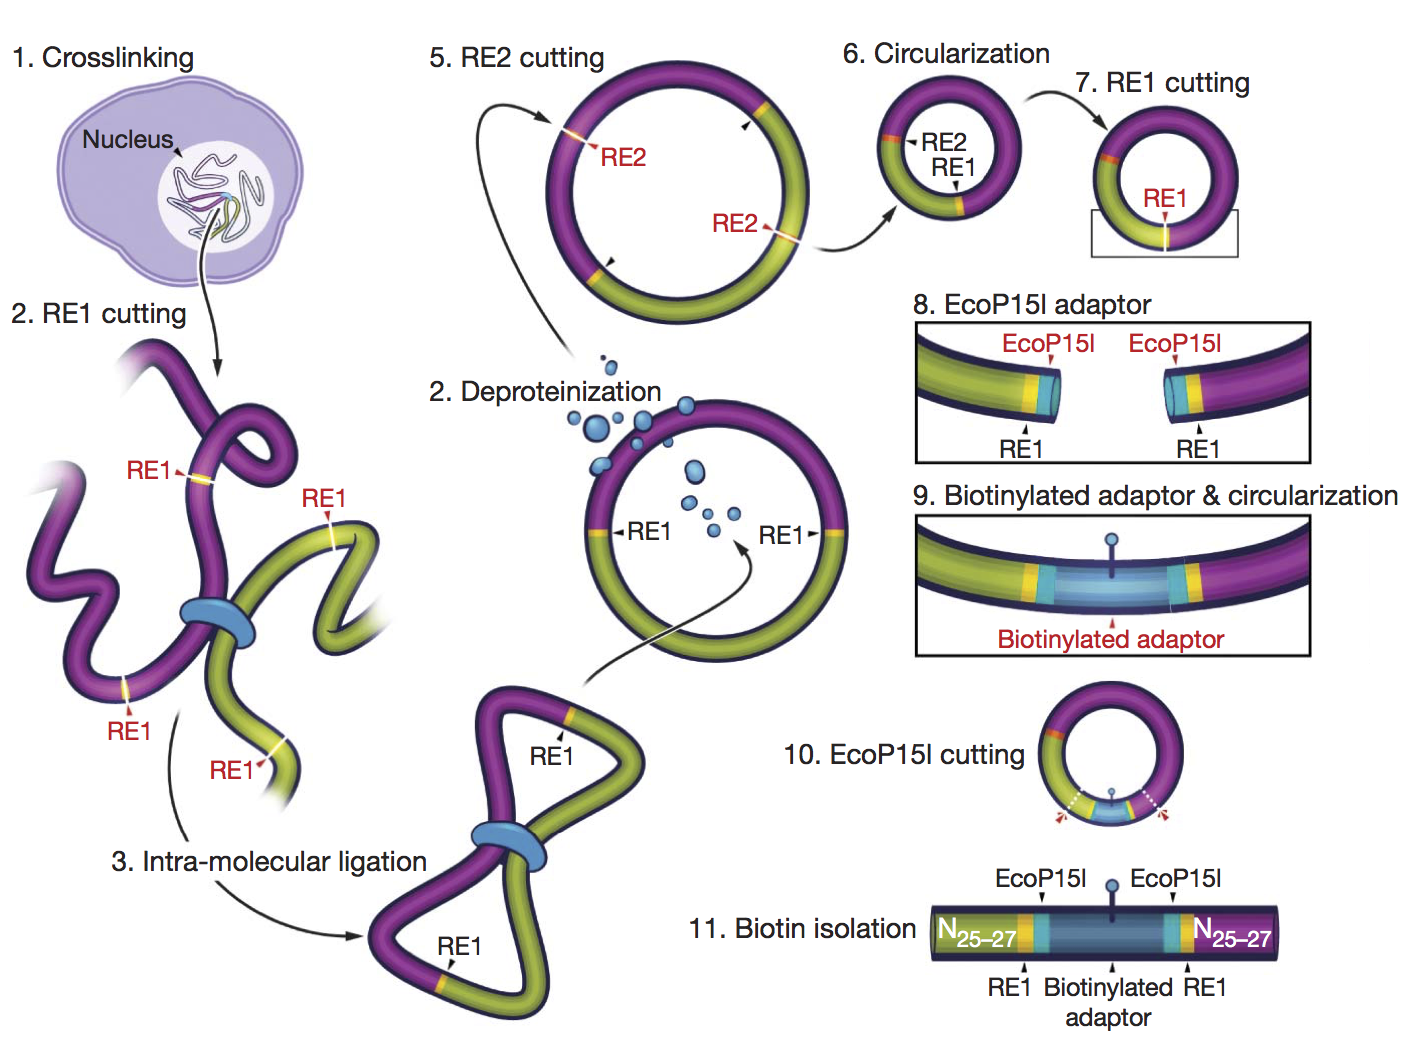
\includegraphics[scale=0.43]{duan.png} \\
% \centering a) $3$C Steps \footnotemark
% \end{minipage}
% \hfill
% \begin{minipage}{.47\textwidth}
%  \includegraphics[scale=0.195]{mousecoheatmap.png} \\
%  \centering b) Interaction Matrix \footnotemark
% \end{minipage}
% \end{figure}

% \begin{itemize}
% \item $3$C is based on restriction fragments cutting and mapping
% \vspace{0.1cm}
% \item Raw data is binned at a given resolution
% \begin{itemize}
% \item 0-100 kb, 100-200 kb, ...
% \end{itemize}
% \end{itemize}

% \footcitetext{duan}
% \footcitetext{dixon2012}

% \end{frame}


% \begin{frame}
% \frametitle{$3$C Deconvolution Problem}

% \large
% \textbf{BUT}
% \normalsize

% \begin{itemize}
% \item $3$C data is obtained over a cell population
% \vspace{0.1cm}
% \begin{itemize}
% \item Each cell has a different interaction matrix.
% \end{itemize}
% \vspace{0.1cm}
% \item Solution over ensemble data is not sufficient:
% \vspace{0.1cm}
% \begin{itemize}
% \item Cells perform different functions in each phase (Temporal)
% \vspace{0.05cm}
% \item Each cell shows different response to the stressors (Spatial) 
% \vspace{0.05cm}
% \item There is also stochasticity
% \end{itemize}
% \end{itemize}

% \end{frame


% \begin{frame}
% \frametitle{$3$C Deconvolution Problem}

% \begin{figure}
% \centering
% \includegraphics[scale=0.25]{subpopulation.png} 
% \end{figure}

% \vspace{-0.6cm}
% \begin{itemize}
% %\item \textbf{Main Question:} Can we unmix $3$C matrices and identify
% %  meaningful latent mixing structures?
% \item \textbf{Main Question:} Given an ensemble $3$C matrix, can we extract the mixing components?
% \end{itemize}

% \vspace{0.3cm}
% Experimental solutions are not perfect:
% \begin{itemize}
% \item Measure the interactions of each single cell~\footfullcite{nagano2013}
% %\begin{itemize}
% %\item Need multiple experiments %to obtain a nice set of representative matrices.
% %\end{itemize} 
% \vspace{0.1cm}
% \item Measure the interactions at a particular cell phase~\footfullcite{naumova2013} %,\footfullcite{Le2013}
% %\begin{itemize}
% %\item Chemicals may disrupt the genome shape
% %\end{itemize} 
% \end{itemize}

% \end{frame}


% % \begin{frame}
% % \frametitle{Why Computational Problem is Important?}

% % \begin{itemize}
% % \item Measure the interaction matrix of each single cell~\footfullcite{nagano2013}
% % \begin{itemize}
% % \item Need multiple experiments %to obtain a nice set of representative matrices.
% % \end{itemize} 
% % \vspace{0.1cm}
% % \item Measure the interactions at a particular cell phase~\footfullcite{naumova2013} %,\footfullcite{Le2013}
% % \begin{itemize}
% % \item Chemicals may disrupt the genome shape
% % \end{itemize} 
% % \end{itemize}

% % \vspace{-0.3cm}
% % \begin{figure}
% % \centering
% % \includegraphics[scale=0.2]{noca.png} \\
% % Nocodazole 
% % \end{figure}

% % \end{frame}


% \begin{frame}
% %\frametitle{Assumptions about Deconvolution}
% \frametitle{Deconvolution Modeling}

% \begin{figure}
% \begin{minipage}{0.47\textwidth}
% \centering
% 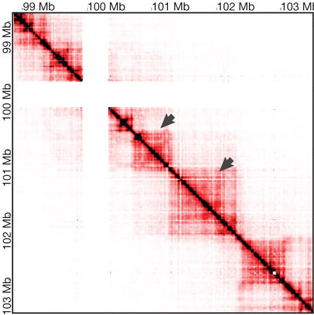
\includegraphics[scale=0.3]{tads.png}~\footnotemark 
% \end{minipage}
% \hspace{0.3cm}
% \begin{minipage}{0.47\textwidth}
% \centering
% \includegraphics[scale=0.25]{../3cplots/decon_ex.png} 
% \end{minipage}
% \end{figure}

% \begin{itemize}
% \item Genome is made up of topological domains~(TADs) 
% \begin{itemize}
% \item highly self-interacting 
% \vspace{0.05cm}
% \item robust consecutive genomic regions 
% \vspace{0.05cm}
% \item building blocks
% \vspace{0.05cm}
% \item few megabases in length
% \end{itemize}
% \end{itemize}

% \footcitetext{nora2012}

% \end{frame}


% \begin{frame}
% \frametitle{Assumptions about Deconvolution}

% \begin{itemize}
% \item Flexible \textit{Bandwidth-quasi-cliques}~({\BQC}'s)
% \end{itemize}

% \begin{figure}
% \centering
% \includegraphics[scale=0.3]{../3cplots/kernel3c.png}
% \end{figure}

% \vspace{-0.3cm}
% \begin{itemize}
% \item Overlapping regions tend to disappear at a single-cell level~\footfullcite{nagano2013}
% \vspace{0.1cm}
% \item Domains are independent of each other
% \vspace{0.1cm}
% \item Domain may not need to be a clique
% %since they become less robust if they share regions with each other.
% \end{itemize}

% \end{frame}


% % \begin{frame}
% % \frametitle{Frequency Deconvolution Problem \FD}

% % %\scriptsize
% % %\begin{problem}[\FD]\label{prob:fd}
% % %We are given an ensemble interaction matrix $\mathbf{F}$, a number of classes $k$, and (optionally) a set of prior domains $P_{c}$. For each class $i$, we want to choose a set of nonoverlapping \textit{bandwidth-quasi-cliques} and density $\lambda_i$ such that the squared Frobenius norm of the difference between $\mathbf{F}$ and the sum of the  matrices $\mathbf{F^i}$ derived from the chosen \textit{bandwidth-quasi-cliques} is minimized.
% % %\end{problem}
% % %\normalsize

% % %\begin{minipage}{0.47\textwidth}
% % \begin{figure}
% % \centering
% % \includegraphics[scale=0.25]{../3cplots/decon_ex.png} 
% % \end{figure}
% % %\end{minipage}


% % \begin{tabular}{cc}
% % \begin{minipage}{0.47\textwidth}
% % \begin{equation*}
% % \mathbf{F} \approx \sum_i \overUnderArrow{$\text{Densities}$}{\lambda_{i}} \overUnderArrow{$\text{Matrices}$}{\mathbf{F^{i}}}
% % \end{equation*}
% % \end{minipage}
% % \hfill
% % \begin{minipage}{0.47\textwidth}
% % \begin{figure}
% % \centering
% % \includegraphics[scale=0.2]{algoblock.png}
% % \end{figure}
% % \end{minipage}
% % \end{tabular}

% % \end{frame}


% \begin{frame}
% \frametitle{A first look at the problem}

% %{\footnotesize
% {\small
% \begin{theorem}\label{th:fdhard}
% \FDint is NP-complete.
% \end{theorem}}

% \vspace{1.5cm}
% Dynamic Programming-based solution:
% \vspace{0.1cm}
% {\small \begin{theorem}\label{th:fdpseudo}
% \FDint can be solved exactly in pseudo-polynomial $O(kn^{4k-1}F_{max}^{k})$ time.
% \end{theorem}}

% \end{frame}

% \begin{frame}
% \frametitle{Approximate Methods}

% % %{\footnotesize
% % {\small
% % \begin{theorem}\label{th:fdhard}
% % \FDint is NP-complete.
% % \end{theorem}

% % \begin{theorem}\label{th:fdpseudo}
% % \FDint can be solved exactly in pseudo-polynomial $O(kn^{4k-1}F_{max}^{k})$ time.
% % \end{theorem}}

% \begin{equation*}
% \mathbf{F} \approx \sum_i \overUnderArrow{$\text{Densities}$}{\lambda_{i}} \overUnderArrow{$\text{Matrices}$}{\mathbf{F^{i}}}
% \end{equation*}

% % \begin{minipage}{0.47\textwidth}
% % \centering
% % \begin{align}
% % & \text{Total number of variables} \notag \\ 
% % & \; = kn(l_{\max} - l_{\min})^{2} \notag
% % \end{align}
% % \end{minipage}
% % \begin{minipage}{0.47\textwidth}
% % \begin{equation*}
% % \mathbf{F} \approx \sum_i \overUnderArrow{$\text{Densities}$}{\lambda_{i}} \overUnderArrow{$\text{Matrices}$}{\mathbf{F^{i}}}
% % \end{equation*}
% % \end{minipage}


% %\begin{itemize}
% %\item We define a variable for each \BQC that represents a domain and bandwidth
% %\end{itemize}
% %A pair $(p,d)$ represents a \BQC by its domain and bandwidth $d$

% %\tiny
% % \scriptsize
% % \begin{align}
% % \text{min}\quad &\overbrace{\sum_{(u,v) \in V^{2}}\,\left(F_{u,v} - \bigg(\sum_{i
% %     \in I} \lambda_{i}\,\big(\sum_{p \in M(u) \cap M(v)}\,\sum_{d=\left|u-v\right|}^{l_{p}-1} x_{pdi}\big)\bigg)
% % \right)^{2}}^{\left\lVert \mathbf{F} - \sum_{i \in
% %     I}\,\lambda_{i}\mathbf{F^{i}} \right\rVert_{F}^{2}}\;\;\;+\;\;\notag \\ 
% % &\; \underbrace{\sum_{i \in I}\,\sum_{(p, d) \in V_{q}} w_{pd}(1-x_{pdi})}_{\text{Domain Weakness}} \;\;\;+\;\;\; \underbrace{\lambda^{p}\,\sum_{i \in I}\,\sum_{p \in P_{c}}\,\sum_{d \in 1, \ldots, l_{p}-1} (1-x_{pdi})}_{\text{Distance From Prior}} \label{eq:deconexobj} \\
% % \text{s.t.}\quad & x_{pdi} + x_{rti} \le 1, 		\qquad\forall \left((p,d), (r,t)\right) \in E_{q},\,\forall i \in I\label{eqn:deconex2} \\
% %                  & x_{pdi} \in \{0, 1\},			\qquad\forall (p,d) \in V_{q},\,\forall i \in I\label{eqn:deconex3}
% % \end{align}
% % %
% % \normalsize

% \begin{figure}
% \centering
% \includegraphics[scale=0.45]{alg1}
% \end{figure}

% \end{frame}


% % %\FDint can be solved exactly in $O(kn^{4k-1}F_{max}^{k})$ time.
% % %\begin{theorem}\label{th:approxset}
% % %\FDint can be approximated to a factor of $3$ via the greedy method for \textit{Set Cover}.
% % %\end{theorem}

% % %\begin{theorem}\label{th:fdhard}
% % %\FDint is NP-complete.
% % %\end{theorem}

% \begin{frame}
% \frametitle{Step$1$: Non-monotone Supermodular Independent Set in Interval Graph}

% %\begin{itemize}
% %\item {\centering
% %\tikz \node (t1) {};}
% %\end{itemize}

% % \begin{minipage}{0.8\textwidth}
% % \centering
% % \begin{align}
% % %& \text{Total number of variables} \notag \\ 
% % %& \; = kn(l_{\max} - l_{\min})^{2} \notag
% % & \text{Total number of variables} = kn(l_{\max} - l_{\min})^{2} \notag
% % \end{align}
% % \end{minipage}

% \tiny
% \begin{align}
% & \text{min}\, Q(X | Y) = \overbrace{\sum_{(u,v) \in V^{2}}\left(F_{u,v} -
%    \bigg(\sum_{i,s \in Y} s\,\big(\sum_{p \in M(u) \cap M(v)}\,\sum_{d=\left|u-v\right|}^{l_{p}-1} x_{pdi}\big)\bigg)
% \right)^{2}}^{\text{Main Objective}} + \overbrace{\sum_{i \in
%   I}\,\sum_{(p, d) \in V_{q}} w^{c}_{pd}(1-x_{pdi})}^{\text{Robustness
%   Prior}} \label{eq:qfunc_s1} \\
% %& \text{min}\, Q(X | Y) = \sum_{(u,v) \in V^{2}}\left(F_{u,v} -
% %   \bigg(\sum_{i,s \in Y} s\,\big(\sum_{p \in M(u) \cap M(v)}\,\sum_{d=\left|u-v\right|}^{l_{p}-1} x_{pdi}\big)\bigg)
% %\right)^{2} \notag \\ 
% %&\hspace{3cm} + \; \sum_{i \in I}\,\sum_{(p, d) \in V_{q}}
% %  w^{c}_{pd}(1-x_{pdi}) \label{eq:qfunc_s1} \\
% & \text{s.t} \quad x_{pdi} + x_{rti} \le 1,\quad \forall \left((p,d), (r,t)\right) \in
% E_{q},\,\forall i \in I \rightarrow \text{Independent Set in Interval
%   Graph} \label{eq:qcons1}  \\
% & \quad \quad x_{pdi} \in \{0, 1\},\quad \forall (p,d) \in
% V_{q},\,\forall i \in I \label{eq:qcons2}
% \end{align}
% \normalsize

% %\begin{tikzpicture}[overlay]
% %      \path[->]<1-> (n1) edge (t1);
% %\end{tikzpicture}

% \centering
% \begin{algorithmic}[1]
% \STATE Solve quadratic LP relaxation
% \STATE Run specialized randomized rounding and remove the intersecting {\BQC}'s
% \end{algorithmic}

% \begin{lemma}\label{lem:step1}
% Step~1 can be approximated to a factor $\frac{1}{e} + (1-\frac{1}{e})\overline{Q}$.
% \end{lemma}

% %\begin{itemize}
% %\item Similar bounds can be achieved by \textit{Set Cover} transformation.
% %\end{itemize}

% \end{frame}


% \begin{frame}
% \frametitle{Step$2$: SDP Relaxation of Binary Least Squares for Density Assignment}

% \begin{itemize}
% \item We define a variable $\forall s \in S^{'} = \{2^{d}\,|\,d \in 1, \ldots, \lfloor \log(F_{max}) \rfloor \}$
% %\begin{itemize}
% %\item More efficient since this removes the assignment constraints.
% %\end{itemize}
% \vspace{0.1cm}
% \item We turn it into a boolean program 
% \end{itemize}

% \vspace{-0.2cm}
% \scriptsize
% \begin{align}
%  \underset{Y}{\text{min}}\quad& \mathbf{y''T}\mathbf{A}\mathbf{y''}
% -2\mathbf{b^{T}}r\mathbf{y''} + \lVert \mathbf{b} \rVert^{2} \label{eq:sdptemp1} \\
% \text{s.t.}\quad &  {y''}_{is}^{2} = 1,\quad i \in 1,\ldots,
% k\,,s \in S' \label{eq:sdptemp2} \\
% &   r^{2} = 1 \label{eq:sdptemp3}
% \end{align}
% \normalsize

% \centering
% \begin{algorithmic}[1]
% \STATE Solve SDP relaxation
% %\STATE Generate $100$ vectors from Multivariate Gaussian $N(0,Y^{*})$
% \STATE Quantize each into the binary vector by their sign 
% \STATE Return $\hat{y} = \min_{l \in 1, \ldots, L}\,\hat{y}_{l}^{T}\mathbf{A}\hat{y}_{l}$.
% \end{algorithmic}

% \begin{lemma}\label{lem:step2}
% Step~2 can be approximated to a factor $\frac{2}{\pi} + (1-\frac{2}{\pi})\overline{Q}$.
% \end{lemma}

% \end{frame}


% \begin{frame}
% \frametitle{\FDfrac}

% \begin{itemize}
% \item We modify only the second step for fractional class densities. 
% \vspace{0.1cm}
% \item Optimally solve the convex quadratic program.
% \end{itemize}

% \scriptsize
% \begin{align}
% & \underset{Y}{\text{min}}\,\sum_{i \in I}\,\sum_{j \in I} \Big(\sum_{(u,v) \in
%   V^{2}}\,m_{ui}m_{vj}\Big)y_{i}y_{j}\;-2\sum_{i \in I}
% \bigg(\sum_{(u,v) \in
%   V^{2}}\,F_{uv}m_{ui}m_{vi}\bigg)y_{i} \label{eqn:fdfracobj} \\
% & y_{i} \ge 0,\quad i \in I\label{eqn:fdfraccons}
% \end{align}
% \normalsize

% \end{frame}


% \begin{frame}
% \frametitle{Exact Deconvolution Methods~(\FDintilp, \FDfracilp)}

% \begin{itemize}
% \item \FDintilp is a convex Quadratic Integer Program~(QIP).
% \vspace{0.15cm}
% \item \FDfracilp is Mixed Integer Quadratic Program~(MIQP).
% \vspace{0.15cm}
% \item Provide an upper bound on the performance.
% \begin{itemize}
% \item Impossible to run the exact methods on larger datasets
% \end{itemize}
% \end{itemize}

% % \tiny
% % \begin{align}
% % &\text{min}\,\sum_{(u,v) \in V^{2}}\,\left(F_{u,v} - \bigg(\sum_{p \in
% %     M[u] \cap M[v]}\,\sum_{d \in 1, \ldots, l_{p}}\,\sum_{i \in
% %     I}\,y_{pdi}\bigg) \right)^{2} + \sum_{i \in I}\,\sum_{(p, d) \in P_{q}} w^{c}_{pdi}x_{pdi} \label{eq:fdexactobj} \\
% % & \text{s.t} \;\; x_{pdi} + x_{rti} \le 1,\quad \forall (p, d), (r, t) \in
% % E_{q},\,\forall i \in I \label{eq:fdexactcons1} \\
% % & \quad \;\; y_{pdi} \le F_{max}\,x_{pdi},\quad \forall (p, d) \in P_{q},\,\forall i \in I\label{eq:fdexactcons2} \\
% % & \quad \;\; -F_{max}(2 - x_{pdi} - x_{rti}) \le y_{pdi} - y_{rti} \le
% % F_{max}(2 - x_{pdi} - x_{rti}), \quad \forall (p, d),(r, t) \notin
% % E_{q},\,\forall i
% % \in I \label{eq:fdexactcons3} \\
% % & \quad \;\; x_{pdi} \in \{0,1\},\quad \forall (p, d) \in P_{q},\,\forall i \in I \label{eq:fdexactcons4} \\
% % & \quad \;\; y_{pdi} \in \{0, 1, \ldots, F_{max}\},\quad \forall (p, d)
% % \in P_{q},\,\forall i \in I \label{eq:fdexactcons5}
% % \end{align}
% % \normalsize

% \end{frame}


% \begin{frame}
% \frametitle{Conclusion}

% \begin{itemize}
% \item We can extract the latent interaction data in $3$C ensemble by deconvolution
% \begin{itemize}
% \item Promising results even without biological priors.
% \end{itemize}
% \vspace{0.1cm}
% \item We return biologically-plausible domain decompositions
% \vspace{0.1cm}
% \item Domain formation is correlated to the epigenetic marker
%   distribution
% \begin{itemize}
% %\item It is not only the markers with insulator roles
% %\vspace{0.1cm}
% \item The direction of causality is yet to be discovered 
% \end{itemize}
% \end{itemize}

% \end{frame}


%===========================================================================
\begin{frame}
\frametitle{Acknowledgements}

\vspace{0.8cm}

\begin{itemize}
\item\textcolor{red}{Thanks to Kingsford Group Members}

\vfill

\begin{figure}

\includegraphics[width=1.3cm]{sloan.jpg} 
\hfill

\includegraphics[width=1.3cm]{moorelogo.png} 
\hfill

\includegraphics[width=1.3cm]{nih.png}
\hfill

\includegraphics[width=1.3cm]{nsf.png}
\hfill

\includegraphics[width=1.2cm]{cmulogo.jpeg} 
\hfill

\includegraphics[width=1.0cm]{cpcblogo.jpeg}
\end{figure}
\vfill

\end{itemize}

\end{frame}


\end{document}
